\section{Results}

\subsection{Duplicate audits and corrected training}

The encoded-byte audit found two cross-split AIDER hash groups. Both had
conflicting labels; excluding every member removed four images and left 6,429.
The Hurricane Damage audit found three cross-split groups with matching labels;
the all-members rule removed six images and left 9,994. No encoded-byte hash
remained in more than one split (Table~\ref{tab:hash-audit}).

\begin{table}[t]
\centering
\caption{Encoded-byte cross-split duplicate audit. Every member of each listed group was excluded before retraining.}
\label{tab:hash-audit}
\begin{tabular}{lrrr}
\toprule
Dataset & Groups & Excluded & Retained \\
\midrule
AIDER & 2 & 4 & 6429 \\
Hurricane Damage & 3 & 6 & 9994 \\
\bottomrule
\end{tabular}
\end{table}


\subsection{Oracle--received protocol gap}

The reference-dependent diagnostic and received-image consistency ranked the
same errors at effective scale 8 but differed in access to finer views. On
AIDER, their mean AUROCs were \(0.964\pm0.013\) and \(0.623\pm0.113\),
respectively. The mean oracle--received AUROC gap was \(0.341\pm0.120\).
On Hurricane Damage, mean AUROC changed from \(0.989\pm0.003\) to
\(0.590\pm0.045\), a gap of \(0.399\pm0.043\).

All six seed-level differences were positive. Every 10,000-replicate paired
bootstrap interval excluded zero: AIDER intervals ranged from
\([0.183,0.249]\) to \([0.415,0.495]\), and Hurricane intervals ranged from
\([0.330,0.378]\) to \([0.413,0.465]\)
(Table~\ref{tab:inflation}). The pre-specified A1 criterion therefore passed.

\begin{table}[t]
\centering
\caption{Paired oracle--received gap in error AUROC. Brackets give 95\% paired bootstrap intervals from 10,000 replicates.}
\label{tab:inflation}
\begin{tabular}{lcc}
\toprule
Seed & AIDER & Hurricane Damage \\
\midrule
101 & 0.351 [0.312, 0.391] & 0.354 [0.330, 0.378] \\
202 & 0.216 [0.183, 0.249] & 0.439 [0.413, 0.465] \\
303 & 0.455 [0.415, 0.495] & 0.405 [0.380, 0.430] \\
\bottomrule
\end{tabular}
\end{table}


Because the two primary protocols also differ in anchor and absolute
degradation regime, we ran a post-hoc mechanism sensitivity that anchors both
scores on \(s=8\) and uses three comparisons. Replacing the unavailable finer
views \(\{1,2,4\}\) with further degradations \(\{16,32,64\}\) produced mean
AUROC gaps of \(0.336\pm0.122\) on AIDER and \(0.398\pm0.044\) on Hurricane
Damage; all six paired intervals remained positive
(Table~\ref{tab:anchor-matched}). This controls anchor and comparison count,
but not degradation direction, and is reported as sensitivity evidence rather
than a new confirmatory endpoint.

\begin{table}[t]
\centering
\caption{Post-hoc anchor-matched mechanism sensitivity. Both scores anchor on the received $s=8$ prediction and use three comparisons; the table reports fine-reference minus further-degradation error AUROC with 95\% paired bootstrap intervals.}
\label{tab:anchor-matched}
\begin{tabular}{lcc}
\toprule
Seed & AIDER & Hurricane Damage \\
\midrule
101 & 0.346 [0.304, 0.387] & 0.351 [0.327, 0.375] \\
202 & 0.209 [0.175, 0.243] & 0.439 [0.413, 0.465] \\
303 & 0.452 [0.411, 0.493] & 0.404 [0.379, 0.429] \\
\bottomrule
\end{tabular}
\end{table}


\subsection{Prospective architecture and operator replication}

The second-architecture replication retained the anchor-matched gap for all
three MobileNetV3-Small seeds and all four operators. Mean MobileNet AIDER gaps
ranged from \(0.215\pm0.014\) (nearest-neighbour) to
\(0.465\pm0.260\) (bicubic). ResNet AIDER means ranged from
\(0.247\pm0.005\) to \(0.336\pm0.122\), and ResNet Hurricane means from
\(0.331\pm0.069\) to \(0.398\pm0.045\)
(Table~\ref{tab:architecture-operator}).

All 36 seed-level intervals across the three architecture/corpus series and
four operators excluded zero. Consequently, pre-specified criteria M1, M2 and
M3 passed. The gap is therefore not conditional on ResNet-18 or bicubic
resampling, although all operators still compare finer and coarser degradation
directions.

\begin{table}[t]
\centering
\caption{Prospective architecture/operator replication of the anchor-matched fine-reference minus received-image error-AUROC gap. Values are mean $\pm$ sample SD over three independently trained seeds.}
\label{tab:architecture-operator}
\resizebox{\textwidth}{!}{%
\begin{tabular}{lccc}
\toprule
Operator & MobileNet AIDER & ResNet AIDER & ResNet Hurricane \\
\midrule
Bicubic & 0.465 $\pm$ 0.260 & 0.336 $\pm$ 0.122 & 0.398 $\pm$ 0.045 \\
Bilinear & 0.420 $\pm$ 0.277 & 0.329 $\pm$ 0.129 & 0.331 $\pm$ 0.069 \\
Nearest & 0.215 $\pm$ 0.014 & 0.251 $\pm$ 0.033 & 0.367 $\pm$ 0.059 \\
Box & 0.244 $\pm$ 0.065 & 0.247 $\pm$ 0.005 & 0.349 $\pm$ 0.079 \\
\bottomrule
\end{tabular}}
\end{table}


\begin{figure}[t]
\centering
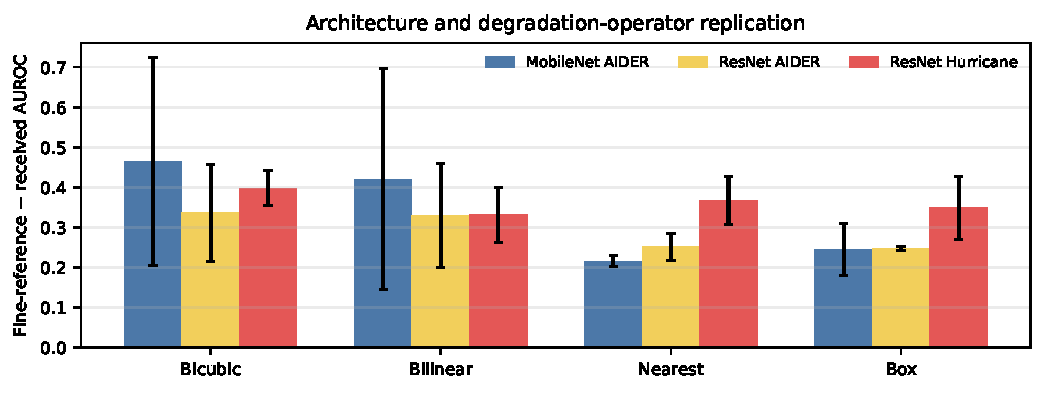
\includegraphics[width=\textwidth]{figures/architecture_operator_replication.pdf}
\caption{Prospective architecture and degradation-operator replication of the
anchor-matched fine-reference minus received-image error-AUROC gap. Bars show
mean across three independently trained seeds; error bars are sample SD.}
\label{fig:architecture-operator}
\end{figure}

\subsection{Fine-reference reveal/mask identification}

Aligned finer views exceeded correspondence-masked finer views in all 24
ResNet corpus/seed/operator combinations. The smallest aligned-minus-masked
mean AUROC gap was 0.359, and the largest empirical one-sided probability was
0.0099. M4 therefore passed.

Mean gaps across seeds ranged from \(0.365\pm0.005\) to
\(0.425\pm0.003\) on AIDER and from \(0.462\pm0.029\) to
\(0.490\pm0.004\) on Hurricane (Table~\ref{tab:reveal-mask}). Because masked
scores preserve the anchor, scale set, score functional, comparison count and
fine-prediction marginals, this result identifies image-specific fine/coarse
correspondence as a driver of the diagnostic advantage within the tested
protocol.

\begin{table}[t]
\centering
\caption{Pre-specified fine-reference reveal/mask experiment. Values are aligned-minus-masked-mean error AUROC across three ResNet seeds; the final column is the maximum empirical one-sided probability across both corpora and all seeds.}
\label{tab:reveal-mask}
\begin{tabular}{lccc}
\toprule
Operator & AIDER gap & Hurricane gap & Max. probability \\
\midrule
Bicubic & 0.371 $\pm$ 0.008 & 0.490 $\pm$ 0.004 & 0.0099 \\
Bilinear & 0.365 $\pm$ 0.005 & 0.469 $\pm$ 0.019 & 0.0099 \\
Nearest & 0.423 $\pm$ 0.006 & 0.482 $\pm$ 0.017 & 0.0099 \\
Box & 0.425 $\pm$ 0.003 & 0.462 $\pm$ 0.029 & 0.0099 \\
\bottomrule
\end{tabular}
\end{table}


\begin{figure}[t]
\centering
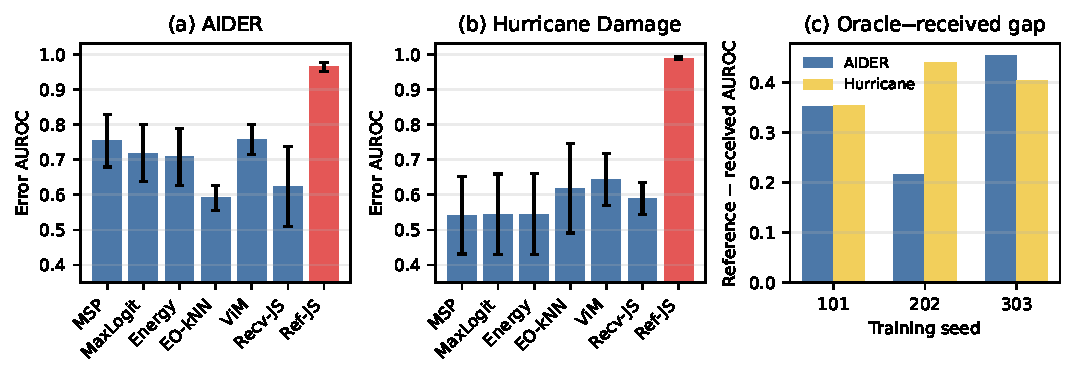
\includegraphics[width=\textwidth]{figures/information_audit.pdf}
\caption{Information-matched error detection. Bars in the first two panels are
mean AUROC across independent training seeds; error bars are sample SD. The red
bar is a non-deployable diagnostic with access to the retained finer reference.
The third panel shows its paired AUROC gap over received-image
consistency for every seed. MSP denotes maximum softmax probability; Recv-JS
and Ref-JS denote received-image and reference-dependent consistency.}
\label{fig:information-audit}
\end{figure}

\subsection{Matched deployable baselines}

Under matched received-image information, no consistency score dominated the
post-hoc baselines (Table~\ref{tab:matched-auroc}). ViM had the highest mean
AIDER AUROC (0.758), closely followed by confidence (0.754); received-image
consistency reached 0.623. On Hurricane Damage, ViM reached 0.643, EO-kNN
0.618, received-image consistency 0.590, and confidence 0.542. These rankings
varied by seed: received-image consistency exceeded confidence strongly for
Hurricane seed 101, was lower for seed 202, and was statistically
indistinguishable for seed 303. The evidence therefore supports the
oracle--received gap, not universal superiority of one deployable
score.

The preregistered paired ViM-minus-EO-kNN comparison was recomputed from
per-example arrays. All three AIDER intervals were positive
(\(0.132\) or greater at the lower bound). On Hurricane Damage, seed 101 was
positive, seed 202 was negative, and seed 303 included zero. ViM therefore did
not dominate EO-kNN across training runs.

\begin{table}[t]
\centering
\caption{Error-detection AUROC under matched received-image information. The final row is a non-deployable diagnostic with access to the retained finer reference. Values are mean $\pm$ sample SD across three independently trained seeds.}
\label{tab:matched-auroc}
\begin{tabular}{lcc}
\toprule
Score & AIDER & Hurricane Damage \\
\midrule
Confidence & 0.754 $\pm$ 0.075 & 0.542 $\pm$ 0.110 \\
Max logit & 0.718 $\pm$ 0.081 & 0.545 $\pm$ 0.114 \\
Energy & 0.708 $\pm$ 0.081 & 0.545 $\pm$ 0.115 \\
EO-kNN & 0.591 $\pm$ 0.035 & 0.618 $\pm$ 0.127 \\
ViM & 0.758 $\pm$ 0.043 & 0.643 $\pm$ 0.074 \\
Received consistency & 0.623 $\pm$ 0.113 & 0.590 $\pm$ 0.045 \\
Reference-dependent diagnostic & 0.964 $\pm$ 0.013 & 0.989 $\pm$ 0.003 \\
\bottomrule
\end{tabular}
\end{table}


\subsection{Threshold transfer}

Native-validation thresholds did not preserve both target coverage and low
selective risk under severe shift. At target coverage 0.70 on AIDER, mean
realised coverage was 0.384 for confidence, 0.257 for ViM, and 0.228 for
received-image consistency. ViM selected a lower-risk subset
(mean selective risk 0.040) but missed the target by 0.443 on average.

On Hurricane Damage, confidence, EO-kNN and ViM mean coverages were 0.029,
0.003 and below 0.001. Received-image consistency instead accepted 0.974 on
average, but its mean selective risk was 0.467. Thus high transferred coverage
did not indicate safe auto-decision retention. Reporting coverage without risk
would reverse the operational interpretation.

\subsection{Intersection-controlled measured-GSD replication}

The guarded CRASAR split retained 1,628 crops from two training sites: 975 for
training, 267 for validation and 386 for internal testing. Exhaustive rectangle
comparison found zero cross-split 512-pixel intersections. Internal test
accuracy was \(0.794\pm0.007\), above the 0.635 majority baseline for every
seed; balanced accuracy was \(0.781\pm0.013\).

The held-out paired evaluation contained 1,441 buildings in 708 UAS spatial
blocks across four acquisitions at three geographies and two hurricane events
(Table~\ref{tab:measured-gsd}).
Same-eligible-label selection retained 531/978 common identifiers at Harlem,
269/366 at McGregor, 337/507 at Mexico Beach 13 October, and 304/634 at Mexico
Beach 14 October. These exclusions are reported because the resulting sample
conditions on cross-product label agreement.
Pooled UAS accuracy was \(0.747\pm0.014\), above the 0.533 pooled majority
baseline for every seed, and balanced accuracy was \(0.752\pm0.014\).
Criterion W11 therefore passed. Satellite accuracy fell to
\(0.486\pm0.081\), below the same majority baseline on average, confirming a
severe cross-platform shift without invalidating the UAS classifier.

The post-hoc joint-overlap sensitivity connected pairs whenever either their
UAS or satellite crops overlapped. It produced two effective clusters at
Harlem and one at each remaining site because the larger satellite footprints
overlap extensively. Pooled intervals continued to include zero, while
site-specific cluster intervals were degenerate and are not interpreted as
independent site inference.

\begin{table}[t]
\centering
\caption{Intersection-controlled CRASAR classifier and pooled held-out paired results. Values are mean $\pm$ sample SD across seeds.}
\label{tab:crasar-summary}
\begin{tabular}{lc}
\toprule
Endpoint & Value \\
\midrule
Guarded internal accuracy & 0.794 $\pm$ 0.007 \\
Guarded internal majority accuracy & 0.635 \\
UAS accuracy & 0.747 $\pm$ 0.014 \\
Satellite accuracy & 0.486 $\pm$ 0.081 \\
Satellite confidence AUROC & 0.465 $\pm$ 0.067 \\
Satellite received-consistency AUROC & 0.614 $\pm$ 0.079 \\
\bottomrule
\end{tabular}
\end{table}

\begin{tabular}{lccccc}
\toprule
Measured GSD & Accuracy & Error conf. & AUROC$_{1-c}$ & AUROC$_{RCG}$ & Lift \\
\midrule
UAS 3.84--4.67\,cm\,px$^{-1}$ & 0.661$\pm$0.040 & 0.782$\pm$0.031 & 0.582$\pm$0.078 & 0.818$\pm$0.030 & 0.236$\pm$0.051 \\
Satellite 30.52\,cm\,px$^{-1}$ & 0.400$\pm$0.170 & 0.800$\pm$0.094 & 0.483$\pm$0.109 & 0.747$\pm$0.126 & 0.264$\pm$0.121 \\
\bottomrule
\end{tabular}


\begin{figure}[t]
\centering
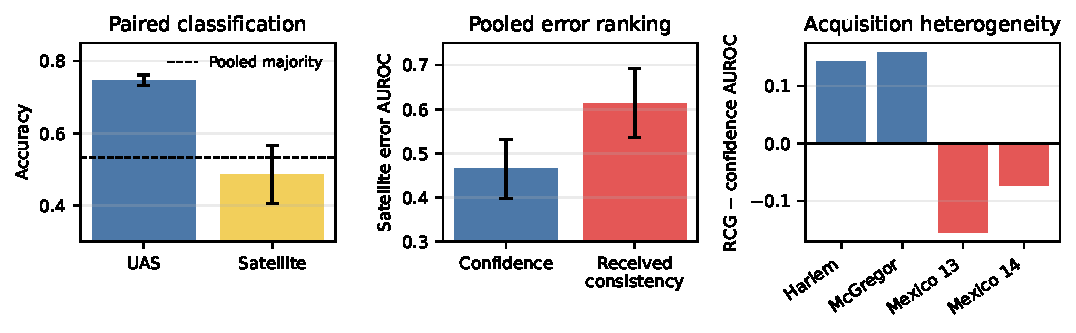
\includegraphics[width=\textwidth]{figures/measured_gsd_audit.pdf}
\caption{Intersection-controlled paired measured-GSD audit. Error bars in the first two
panels are sample SD across training seeds. The acquisition panel shows that the
pooled received-consistency advantage is confined to the two Hurricane Ian
sites and reverses at both held-out Hurricane Michael sites.}
\label{fig:measured-gsd}
\end{figure}

\subsection{Measured-GSD ranking and threshold transfer}

On pooled satellite views, received-image consistency reached error AUROC
\(0.614\pm0.079\), compared with \(0.465\pm0.067\) for confidence; all three
seed differences were positive and the mean difference was 0.149. This pooled
summary did not generalise by site. Mean differences were 0.143 at Harlem
Heights and 0.159 at McGregor, but \(-0.155\) and \(-0.073\) on the two
Mexico Beach sites. The paired spatial-cluster bootstrap intervals for the
pooled difference included zero for every seed. W12 therefore failed.

Measured threshold transfer was also heterogeneous. At target coverage 0.70,
received-image consistency achieved mean satellite coverage
\(0.701\pm0.138\), compared with \(0.499\pm0.068\) for confidence. Mean
selective risk was lower (0.456 versus 0.548), but seed 202 reversed this
ordering (0.549 versus 0.530), and spatial-cluster risk-difference intervals
included zero. The preregistered mean-based W13 therefore passed, while the
stricter post-hoc all-seed robustness sensitivity failed. The expanded
evaluation changes the conclusion from a positive two-site ranking result to
event-associated heterogeneity with no confirmatory ranking success and no
seed-uniform threshold-transfer robustness.

\subsection{Third-event Hurricane Idalia sensitivity}

The prospective third-event sensitivity retained 458/605 common Steinhatchee
River building identifiers with matching eligible UAS/crewed-aircraft labels.
Measured GSD was 12.70 and 15.02 cm\,px\(^{-1}\), so the 512-pixel crops span
approximately 65.0 and 76.9 m. Joint UAS/crewed overlap grouping yielded 37
clusters.

Mean held-out UAS balanced accuracy was 0.572, passing E1; absolute accuracy
remained below the 0.954 majority baseline because only 21 paired buildings
were damaged. E2 passed with complete raw outputs and cluster inference.
Received consistency exceeded confidence on crewed-aircraft errors by 0.312,
0.389 and 0.274 AUROC across seeds; all three 2,000-replicate cluster intervals
excluded zero and mean lift was 0.325 (Table~\ref{tab:idalia}). Accuracy
improved slightly for seed 101 and declined for seeds 202 and 303, consistent
with the pre-specified absence of an accuracy-direction criterion.

\begin{table}[t]
\centering
\caption{Prospective third-event Hurricane Idalia sensitivity on 458 same-building UAS/crewed-aircraft pairs. The final columns report received-consistency minus confidence error-AUROC and its joint-overlap-cluster bootstrap interval.}
\label{tab:idalia}
\begin{tabular}{lrrrr}
\toprule
Seed & UAS balanced acc. & Crewed balanced acc. & AUROC lift & 95\% CI \\
\midrule
101 & 0.593 & 0.621 & 0.312 & [0.261, 0.372] \\
202 & 0.527 & 0.578 & 0.389 & [0.210, 0.472] \\
303 & 0.596 & 0.570 & 0.274 & [0.142, 0.344] \\
\bottomrule
\end{tabular}
\end{table}

